\section{Bounded inversion}
\label{sec:inverse}

\subsection{The guard}
\label{sec:guard}

The solver does not need $d(p)$ everywhere. Coverage is computed as
$1-\mathrm{smoothstep}(h-a,\,h+a,\,d)$ for stroke half-width $h$ and
antialiasing width $a$ (Eq.~\ref{eq:alpha}), so any $d$ above $h+a$ produces
identical output. We therefore fix a \emph{guard}
\begin{equation}
  G \;=\; \max\bigl(h+a,\ \tfrac{3}{4}s\bigr)
  \label{eq:guard}
\end{equation}
and require only
\begin{equation}
  \tilde d(p) \;=\; \min\bigl(d(p),\, G\bigr).
  \label{eq:clamped}
\end{equation}
Everything below is exact with respect to~\eqref{eq:clamped}, which is exact with
respect to the image: the clamp is the renderer's own quantization, and it
changes no output pixel. (The envelope and ratio views of
\S\ref{sec:envelope}--\S\ref{sec:visibility} need the field measured a whole
pitch out rather than a stroke width out, so under those views the solver runs
with $G$ widened to $\max(h+a,\,s)$; every bound below holds verbatim at the
wider value.)

Two smaller consequences of the same observation come free. The solver takes an
\emph{accept} threshold $h-a$: once a residual falls
below it the pixel is fully inked and the loop can stop, whatever else is nearby.
And it takes $G$ itself as a \emph{reject} threshold, which is what makes the
interval below finite.

\subsection{The drift constant}
\label{sec:drift}

Everything turns on how fast ring $n$'s boundary can outrun its own radius. Using
(P3) on~\eqref{eq:qn},
\begin{equation}
  \rad(q_n) \;=\; \rad\bigl(\Rot{-n\theta}p - n\delta\bigr)
    \;\le\; \rad\bigl(\Rot{-n\theta}p\bigr) + n\,\rad(-\delta),
  \label{eq:driftup}
\end{equation}
so the per-index rate is exactly
\begin{equation}
  m \;=\; \rad(-\delta),
  \label{eq:drift}
\end{equation}
the support value of the metric in the direction \emph{opposite} the walk. The
obvious bound is $m \le \lVert\delta\rVert$, and $\lVert\delta\rVert$ is what a
first implementation naturally uses. But~\eqref{eq:drift} is smaller, sometimes
much smaller: $m=\max(|\delta_x|,|\delta_y|)$ for a square, and as little as
$\lVert\delta\rVert/2$ for a triangle whose flat side leads the walk (the
vertex trailing); with the vertex leading, $m=\lVert\delta\rVert$ and nothing
is gained.

The same number has a physical face: Corollary~\ref{cor:mach} says the family
folds exactly when $m>s$, so $m$ is the Mach number of the walk, and the
solver constants below are the search-side shadow of the fold law.

The gap is not cosmetic. Section~\ref{sec:window} shows the search interval is
finite if and only if $m \neq s$, with width $\propto 1/|s-m|$. Substituting
$\lVert\delta\rVert$ for $m$ therefore declares an entire band of settings
unbounded that are in fact tightly bounded, and a solver that falls back to
subsampling on that band produces the failure in Figure~\ref{fig:drift}: not holes,
but a wholesale thinning that removes two thirds of the ink and looks, to a user,
like the pattern has changed. It is the largest single fidelity error we measured
from any cause ($\artDriftLooseDiff\%$ of pixels), and it comes from a bound that
is merely loose rather than wrong.

\subsection{A provably sufficient interval of indices}
\label{sec:window}

\begin{figure*}[t]
  \centering
  \begin{subfigure}[t]{0.485\textwidth}
    \vspace{0pt}
    \begin{tikzpicture}
      \begin{axis}[paperaxis, scale only axis, width=6.4cm, height=4.2cm, name=resax,
        xlabel={ring index $n$}, ylabel={residual $h_p(n)$},
        xmin=0, xmax=74, ymin=-260, ymax=380,
        legend style={at={(0.5,-0.36)}, anchor=north, draw=none, fill=none,
                      /tikz/every even column/.append style={column sep=0.45cm}},
        legend columns=2,
      ]
        % window shading
        \addplot[draw=none, fill=cool!10, forget plot] coordinates
          {(\figLo,-260) (\figHi,-260) (\figHi,380) (\figLo,380)} \closedcycle;
        % guard band
        \addplot[draw=none, fill=accent!22, forget plot] coordinates
          {(0,-10.5) (74,-10.5) (74,10.5) (0,10.5)} \closedcycle;
        \addplot[cool, thick, dashed] table [x=n, y=upper, col sep=comma] {data/residual.csv};
        \addlegendentry{upper envelope $r + n(m-s)$}
        \addplot[warm, thick, dashed] table [x=n, y=lower, col sep=comma] {data/residual.csv};
        \addlegendentry{lower envelope $\kappa|r-nL| - ns$}
        \addplot[ink, very thick] table [x=n, y=h, col sep=comma] {data/residual.csv};
        \addlegendentry{$h_p(n)$}
        \addplot[only marks, mark=*, mark size=1.9pt, accent]
          table [x=n, y=h, col sep=comma] {data/residual-visited.csv};
        \addlegendentry{evaluated (\figEvals)}
        \draw[soft, dashed] (axis cs:\figNaive,-260) -- (axis cs:\figNaive,380);
        \node[soft, font=\scriptsize, anchor=south, rotate=90] at (axis cs:\figNaive,-250) {naive $r/s$};
      \end{axis}
      \path ([yshift=8pt]resax.north);
    \end{tikzpicture}
    \caption{The residual at one pixel.}
    \label{fig:residual}
  \end{subfigure}\hfill
  \begin{subfigure}[t]{0.485\textwidth}
    \vspace{0pt}
    \begin{tikzpicture}
      \begin{axis}[paperaxis, scale only axis, width=6.4cm, height=4.2cm, name=fanax,
        xlabel={$\lVert p\rVert$ (world units, $s=14$)}, ylabel={indices},
        xmin=0, xmax=1600, ymin=0, ymax=82,
        legend style={at={(0.5,-0.36)}, anchor=north, draw=none, fill=none,
                      /tikz/every even column/.append style={column sep=0.45cm}},
        legend columns=2,
      ]
        \addplot[accent, very thick] table [x=radius, y=stray, col sep=comma] {data/fan-triangle.csv};
        \addlegendentry{worst stray of $n^\star$}
        \addplot[cool, thick, densely dashed] table [x=radius, y=span, col sep=comma] {data/fan-triangle.csv};
        \addlegendentry{proven interval}
        \addplot[warm, thick] table [x=radius, y=evaluated, col sep=comma] {data/fan-triangle.csv};
        \addlegendentry{indices we evaluate}
        \addplot[soft, thin, dotted, domain=0:1600, samples=2] {16};
        \addlegendentry{$\pm16$ budget}
      \end{axis}
      \path ([yshift=8pt]fanax.north);
    \end{tikzpicture}
    \caption{Worst-case stray against radius.}
    \label{fig:fan}
  \end{subfigure}
  \Description{Two plots. The left plots the residual against ring index: a steeply
  falling dark curve crosses zero near index forty-one, bracketed above and below by
  two dashed straight lines, with a pink horizontal guard band around zero and a
  shaded vertical strip marking the certified index interval; nine dots on the curve
  mark the indices actually evaluated, widely spaced far from the crossing and
  closely spaced near it. The right plots four quantities against radius: the worst
  stray of the nearest index grows roughly linearly past sixty, the proven interval
  width grows with it, the count of indices evaluated stays near ten, and a dotted
  horizontal line at sixteen marks a fixed budget that the stray crosses early.}
  \caption{\figlead{Certifying and skipping the index interval.}
  \textbf{(a)}~The residual at one pixel is sandwiched between two lines in $n$,
  which is enough to certify a finite interval. The naive index guess is
  $\figNaive$; the true nearest ring is $\figTrue$, $\figGap$ rings away and
  outside any small neighborhood. The two envelopes of Lemma~\ref{lem:envelope}
  cross the guard band (pink) at $\figLo$ and $\figHi$, proving that no ring
  outside those $\figSpan$ indices comes within $G$; the Lipschitz rule then
  visits $\figEvals$ of them (dots), taking long strides while $|h|$ is large
  and closing in only near the crossing. \textbf{(b)}~Why no fixed interval
  could have been enough, measured. Triangles, $\theta=0.02$, $96$ directions
  per radius; the stray is the worst seen out to that radius. The nearest index
  leaves any fixed neighborhood of the naive guess and the gap grows linearly,
  so a budget is a horizontal line that the requirement crosses, here at
  $r\approx500$, a third of the way across the frame. The proven interval grows
  too, since the rings near a pixel genuinely become more numerous, but the
  Lipschitz skip keeps what we evaluate well below it.}
  \label{fig:bounds}
\end{figure*}

Write $r=\lVert p\rVert$, $L=\lVert\delta\rVert$, $m=\rad(-\delta)$, and note
$\rad(\Rot{-n\theta}p)\le r$ by (P2) and
$\lVert q_n\rVert \ge |r - nL|$ by the triangle inequality on~\eqref{eq:qn};
both are independent of $\theta$.

\begin{lemma}[Two-sided envelope]
\label{lem:envelope}
For all $n \ge 0$ and all $\theta$,
\begin{equation}
  \max\bigl\{\, \kappa\,|r - nL|,\ \ nm - r \,\bigr\} - (ns+\varphi)
  \ \le\ h_p(n)\ \le\ r + nm - (ns+\varphi).
  \label{eq:envelope}
\end{equation}
\end{lemma}

\begin{proof}
The upper bound is~\eqref{eq:driftup} with $\rad(\Rot{-n\theta}p)\le r$. For the
first lower bound, (P2) gives $\rad(q_n) \ge \kappa\lVert q_n\rVert \ge
\kappa|r-nL|$. For the second, subadditivity applied as
$\rad(-n\delta) \le \rad(q_n) + \rad(-\Rot{-n\theta}p)$ gives
$\rad(q_n) \ge nm - r$. Subtract $ns+\varphi$ throughout.
\end{proof}

Both bounds are affine in $n$ (the first piecewise so), so intersecting them with
the guard band $|h|\le G$ yields an interval by inspection.

\begin{theorem}[Sufficient interval]
\label{thm:window}
Let
\begin{equation}
  n_{\mathrm{lo}} = \max\left(0,\ \left\lfloor \frac{\kappa r - \varphi - G}{s + \kappa L} \right\rfloor\right),
  \qquad
  n_{\mathrm{hi}} = \left\lceil \frac{r + \varphi + G}{|s - m|} \right\rceil .
  \label{eq:window}
\end{equation}
If $m \neq s$, then every $n$ with $|h_p(n)| \le G$ satisfies
$n_{\mathrm{lo}} \le n \le n_{\mathrm{hi}}$, and consequently
\begin{equation}
  \tilde d(p) \;=\; \min\Bigl(G,\ \min_{n_{\mathrm{lo}} \le n \le n_{\mathrm{hi}}} |h_p(n)|\Bigr).
  \label{eq:exact}
\end{equation}
\end{theorem}

\begin{proof}
For the lower end, note first that every $n < n_{\mathrm{lo}}$ lies on the
branch $nL\le r$ automatically: $n(s+\kappa L) < \kappa r - \varphi - G \le
\kappa r$ gives $\kappa nL < \kappa r$. On that branch \eqref{eq:envelope}
gives $h_p(n) \ge \kappa r - \kappa nL - ns - \varphi > G$, so
$|h_p(n)| > G$ and no index below $n_{\mathrm{lo}}$ is admitted. For the upper
end, if $s>m$ then $h_p(n) \le r + n(m-s) - \varphi$, and $h_p(n)\ge -G$ forces
$n \le (r - \varphi + G)/(s-m)$; if $m>s$ then $h_p(n) \ge n(m-s) - r - \varphi$,
and $h_p(n)\le G$ forces $n \le (r + \varphi + G)/(m-s)$. Both are bounded
by~\eqref{eq:window}. Every excluded index has $|h_p(n)|>G$, so it cannot lower
the clamped minimum, giving~\eqref{eq:exact}.
\end{proof}

Three remarks. First, \emph{$\theta$ does not appear} in~\eqref{eq:window}. The
rotation destroys the closed form but does not widen the search: it is bounded
away by $\rad(\Rot{-n\theta}p)\le r$, which is tight since some index does place
$p$ along a vertex direction. Second, the interval is tight in the sense that both
envelope constants are attained, so it cannot be narrowed without using more than
$\rad$'s convexity class. Third, the interval degenerates only on the single locus
$m=s$: there, the two envelopes are parallel to the guard band and infinitely many
rings genuinely pass within $G$ of a generic point. That is not a failure of the
bound but a property of the family, and we return to it in
Sections~\ref{sec:closed} and~\ref{sec:limits}.

Figure~\ref{fig:residual} works one pixel through. The naive guess is $\figNaive$;
the truth is $\figTrue$, $\figGap$ rings away. The proven interval is
$[\figLo,\figHi]$, and Figure~\ref{fig:fan} shows why no constant would have done:
we measured how far the nearest index actually strays from the naive guess, worst
case over directions, and it grows linearly in $r$: past $r\approx500$ it
exceeds the widest neighborhood our previous solver could even express. The same
plot confirms the theorem empirically: over $\winChecks$ sampled pixels whose
nearest ring is inside the guard, the argmin fell inside~\eqref{eq:window} every
time.

\subsection{Skipping the interval}
\label{sec:skip}

An interval is a proof, not yet an algorithm; near the origin it is a handful of
indices, but at zoom-out it can be thousands. We shrink it with a Lipschitz
argument in index space.

\begin{lemma}[Index Lipschitz bound]
\label{lem:lipschitz}
For all $n, n'\ge 0$,
$|h_p(n')-h_p(n)| \le \Lambda\,|n'-n|$ with
\begin{equation}
  \Lambda \;=\; s + L + |\theta|\,r .
  \label{eq:lambda}
\end{equation}
\end{lemma}

\begin{proof}
By (P1), $|\rad(q_{n'})-\rad(q_n)| \le \lVert q_{n'}-q_n\rVert$. From
\eqref{eq:qn}, $\lVert q_{n'}-q_n\rVert \le
\lVert(\Rot{-n'\theta}-\Rot{-n\theta})p\rVert + |n'-n|L
= 2r\bigl|\sin\tfrac{(n'-n)\theta}{2}\bigr| + |n'-n|L
\le |n'-n|\,(|\theta| r + L)$. The ring radius contributes $s|n'-n|$.
\end{proof}

So from a sample with residual $|h_p(n)| = v$ and a current best $b$, no index
within $(v-b)/\Lambda$ of $n$ can beat $b$, and the whole run can be skipped
unevaluated. This is sphere tracing~\cite{Hart1996Sphere} with the ray replaced by the
index axis. The loop is Algorithm~\ref{alg:scan}.

\begin{algorithm}[t]
\caption{Ring scan, given $p$, the family parameters, the budget $B$, the guard
$G$, and the accept threshold $h-a$. With
$\mathrm{span}=n_{\mathrm{hi}}-n_{\mathrm{lo}}+1$, exact when
$\mathrm{span}\le B$ (Theorem~\ref{thm:window}).}
\label{alg:scan}
\begin{algorithmic}[1]
\State $[n_{\mathrm{lo}}, n_{\mathrm{hi}}] \gets$ interval from \eqref{eq:window};
       $\Lambda \gets s + L + |\theta| r$
\State $\sigma \gets 2^{\max(0,\,\lceil \log_2(\mathrm{span}/B) \rceil)}$ \Comment{$1$ when the interval fits}
\State $n \gets \sigma\lceil n_{\mathrm{lo}}/\sigma \rceil$ \Comment{anchored to the global lattice, not to $p$}
\State carry $\cos(n\theta-\arg p)$, $\sin(n\theta-\arg p)$, $n\delta$, $ns+\varphi$
\State $b \gets \infty$
\For{$B$ iterations, while $n \le n_{\mathrm{hi}}$}
  \State $v \gets |\rad(q_n) - (ns+\varphi)|$ \Comment{no transcendentals}
  \State $b \gets \min(b, v)$
  \State \textbf{if} $b \le$ accept \textbf{then return} $b$
  \State $j \gets \sigma\max\bigl(1, \lceil (\lfloor (v - \min(b,G))/\Lambda \rfloor + 1)/\sigma \rceil\bigr)$
  \State advance the carried quantities by $j$; $n \gets n + j$
\EndFor
\State \Return $\min(b, G)$
\end{algorithmic}
\end{algorithm}

Two implementation points matter enough to measure (Table~\ref{tab:ablation}).

\emph{Carried motion.} $q_n$ advances by a fixed rotation and a fixed translation
per index, so the loop carries $\cos(n\theta-\arg p)$ and $\sin(n\theta-\arg p)$
through an angle-addition step instead of recomputing them. Combined with the
transcendental-free forms in~\eqref{eq:metrics}, the inner iteration contains no
transcendental function at all: it is a handful of multiplies, a max, and an
absolute value. We re-anchor every $32$ carried steps, which keeps
\texttt{f32} drift far below a pixel; at large $n$ the carried value is in fact steadier than
$\cos(n\theta-\alpha)$ evaluated cold, because the argument does not grow.

\emph{Lattice anchoring.} When the interval exceeds the budget $B$ we stride by a
power of two, and the start is snapped to a multiple of the stride rather than to
$n_{\mathrm{lo}}$. Since $n_{\mathrm{lo}}$ depends on $p$ and the stride does not,
this is the difference between neighboring pixels agreeing on \emph{which rings
exist} and each pixel sampling its own subset. Section~\ref{sec:limits} shows the
consequence, which is severe and free to avoid.

\subsection{Translated polygons in closed form}
\label{sec:closed}

\begin{figure}[t]
  \centering
  \begin{tikzpicture}
    \begin{axis}[paperaxis, height=5.3cm,
      xlabel={ring index $n$}, ylabel={$h_p(n)$},
      xmin=0, xmax=64, ymin=-700, ymax=440,
      ytick={-600,-400,-200,0,200,400},
      legend style={at={(0.5,-0.40)}, anchor=north, draw=none, fill=none,
                    /tikz/every even column/.append style={column sep=0.45cm}},
      legend columns=2,
    ]
      % Zero is a line, not a band: at this scale a band wide enough to see would
      % be wider than the crossing it marks.
      \addplot[accent, thin, forget plot] coordinates {(0,0) (64,0)};
      \addplot[cool, very thick] table [x=n, y=h, col sep=comma] {data/convex-shrinking.csv};
      \addlegendentry{$m < s$: one crossing}
      % Dashed, not for emphasis: the two residuals very nearly coincide until the
      % second facet, and a solid line drawn second would simply hide the first.
      \addplot[warm, very thick, densely dashed] table [x=n, y=h, col sep=comma] {data/convex-marginal.csv};
      \addlegendentry{$m = s$: flat forever}
      % Where one facet hands over to the next, from the same data the curves use.
      \addplot[cool, only marks, mark=*, mark size=1.5pt, mark options={fill=white, thick},
               forget plot] table [x=n, y=h, col sep=comma] {data/convex-shrinking-breaks.csv};
      \addplot[warm, only marks, mark=*, mark size=1.5pt, mark options={fill=white, thick},
               forget plot] table [x=n, y=h, col sep=comma] {data/convex-marginal-breaks.csv};
      \node[anchor=north east, inner sep=1.5pt, fill=white, draw=cool, semithick]
        at (rel axis cs: 0.615, 0.97) {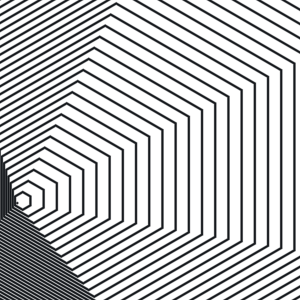
\includegraphics[width=1.62cm]{figures/inset-convex-cross.png}};
      \node[anchor=north east, inner sep=1.5pt, fill=white, draw=warm, semithick]
        at (rel axis cs: 0.985, 0.97) {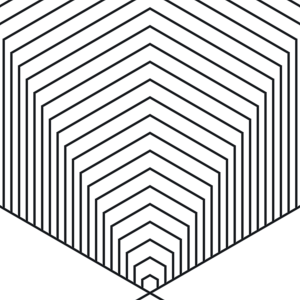
\includegraphics[width=1.62cm]{figures/inset-convex-flat.png}};
    \end{axis}
  \end{tikzpicture}
  \Description{A plot of the residual against ring index for two settings, with a
  thin horizontal line at zero. Both curves start near four hundred and fall. The
  blue curve is visibly made of four straight pieces of decreasing steepness, with
  small hollow circles where one piece meets the next; it crosses zero once, part
  way along its second piece, and keeps descending. The orange curve falls through
  three pieces and then levels onto a horizontal line, which it holds for the rest
  of the plot. Two small framed thumbnails at the top right show the two walking
  hexagon families the curves belong to.}
  \caption{With $\theta=0$ the residual of a translated polygon is convex and
  piecewise linear in $n$, one segment per facet (hexagon, $s=14$); the hollow
  circles mark the handovers. When the drift is below the spacing (blue, $m=10$)
  it falls monotonically and crosses zero once, on some facet's own segment, so
  the answer is a linear solve. At the marginal drift $m=s$ (orange) the leading
  facet's slope cancels and the residual is \emph{constant} past the crossover:
  all large indices are exactly equidistant, so no enumeration of finite length
  can settle them. One evaluation of the constant settles all of them at once.
  The insets are these same two families, framed in each curve's color: below the
  marginal drift the walking hexagons stay a drawing; at it the far side piles
  into a plateau. Both curves are shown on the query point of
  Table~\ref{tab:cost}'s hexagon setting; the point and the drift are deliberately
  not parallel, since a $p$ collinear with $\delta$ keeps one facet active for
  every $n$ and would draw a single straight line here.}
  \label{fig:convex}
\end{figure}

The scan of Algorithm~\ref{alg:scan} is exact and fast, but for $\theta=0$ the
scan can be replaced by an exact $O(N)$ solution regardless of the interval
width, including on the locus where the interval is infinite. Property (P4) is the reason,
and we have not found it used for this.

With $\theta=0$, \eqref{eq:qn} becomes affine in $n$: $q_n = p - n\delta$. Writing
$a_k = \langle p, u_k\rangle$ and $b_k = \langle \delta, u_k\rangle$ over the $N$
unit normals,
\begin{equation}
  h_p(n) \;=\; \max_{k}\,(a_k - n b_k) \;-\; ns - \varphi ,
  \label{eq:convex}
\end{equation}
a maximum of $N$ affine functions of $n$ minus an affine function: convex and
piecewise linear, with at most $N$ breakpoints and slopes increasing in $n$. Its
asymptotic slope is $m - s$ with $m=\rad(-\delta)=\max_k(-b_k)$: the same drift
constant as~\eqref{eq:drift}, arrived at independently.

\begin{proposition}
\label{prop:closed}
Let $\theta=0$, let the shape be a polygon with $N$ facets, and let $p$ lie on
or outside the innermost ring, $\rad(p)\ge\varphi$. (Inside it, $h_p$ is
negative and strictly decreasing, so the answer is
$\min(G,\,\varphi-\rad(p))$, attained at $n=0$.)
\begin{enumerate}
  \item If $m < s$, $h_p$ is strictly decreasing and has exactly one zero, which
  lies on some facet's own linear segment. That zero is one of the $N$ solves
  $n_k = (a_k-\varphi)/(s+b_k)$, and
  $\tilde d(p) = \min(G,\min_k \min_{j\in\{\lfloor n_k\rfloor, \lfloor n_k\rfloor+1\}} |h_p(j)|)$,
  with each candidate clamped to $j\ge0$: an unclamped negative candidate
  indexes a ring that does not exist.
  \item If $m = s$, the facet $k^\star$ attaining $m$ has $s + b_{k^\star} = 0$
  (its solve is skipped), and $h_p \equiv a_{k^\star} - \varphi$ on the terminal
  segment, attained at every index past the crossover. $\tilde d(p)$ is the
  minimum of $|a_{k^\star}-\varphi|$ against the remaining facets' clamped
  candidates as in (1), then clamped at $G$.
\end{enumerate}
In both cases the cost is $2N+2$ evaluations of~\eqref{eq:convex}, independent of
$r$, $s$, and $\delta$.
\end{proposition}

\begin{proof}
By~\eqref{eq:convex} $h_p$ is convex with slopes $-(s+b_k)$ ordered increasingly
in $n$. If $m<s$ then $s + b_k > 0$ for every $k$, so every slope is negative and
$h_p$ is strictly decreasing; being continuous with $h_p(0)=\rad(p)-\varphi\ge0$
by hypothesis and $h_p\to-\infty$, it has one zero, attained
on whichever segment is active there, whose linear equation is
$a_k - nb_k - ns - \varphi = 0$. Convexity makes $|h_p|$ unimodal, so its integer
minimum is adjacent to the real zero. If $m=s$, the maximum in~\eqref{eq:convex}
is eventually attained by $k^\star$, and there
$h_p(n) = a_{k^\star} + ns - ns - \varphi$ is constant; before the crossover
$h_p$ is a strictly decreasing piecewise-linear function whose zero, if it has
one, is covered by the remaining facets' candidates.
\end{proof}

The square case ($N=4$, normals on the axes) is presumably folklore; the content
of Proposition~\ref{prop:closed} is that it generalizes to every side count
and, more importantly, that case (2) exists.
Figure~\ref{fig:convex} plots both. The marginal case is the one that repays the
effort: it is exactly the locus where Theorem~\ref{thm:window} gives up, it is
the sonic boundary of Corollary~\ref{cor:mach} --- the walk that matches its
own growth, rings piling into a plane wake --- and it is
not exotic. It is the family whose rings pile up along a line, which is a
pattern users deliberately make. Any scan, of any budget, walks off the end of
that flat segment without reaching the indices that carry the answer. Handling it
costs one comparison. Table~\ref{tab:ablation} measures the difference at
$\ablClosedMarginal\times$.

We dispatch to the cheapest sufficient method: constant-time \texttt{mod} when
$\delta=0$ and ($\theta=0$ or the shape is a circle, since rotating a radial
metric is a no-op --- for circles alone, by
Corollary~\ref{cor:rotation}); the quadratic for translated circles; Proposition~\ref{prop:closed}
for translated polygons with integral side count and $m \le s$;
Algorithm~\ref{alg:scan} otherwise. A morph that passes through fractional side
counts is not any polygon's support function, so it correctly falls through to the
scan rather than solving for facets that do not exist.

\subsection{Implementation}
\label{sec:impl}

The solver exists twice: once in TypeScript for tests and once in WGSL for the
renderer, generated as separate functions and composed as shader
includes~\cite{WebGPU}. The twins are checked against each other numerically on
the GPU (Section~\ref{sec:protocol}) and the TypeScript side is checked against
brute force in a unit test that sweeps shapes, spacings, offsets, and radii,
including the marginal drift. Ring evaluation is branch-light: the interval, the
stride, and $\Lambda$ are computed once per pixel, and the loop body has a single
data-dependent branch (the accept exit).

We set $B=1024$ evaluations and additionally cap the interval span at $2^{16}$ so
that the loop terminates on the $m=s$ locus when the closed form does not apply
($\theta\neq0$). Neither constant affects correctness where
Theorem~\ref{thm:window} applies; both are reported and ablated in
Section~\ref{sec:results}. Three numerical points. The shipped upper bound uses
the two per-branch forms derived inside the proof of
Theorem~\ref{thm:window}, $(r-\varphi+G)/(s-m)$ and $(r+\varphi+G)/(m-s)$,
which are slightly tighter than the single display \eqref{eq:window}. The
closed-form dispatch admits $m \le s + 10^{-4}$, and within $10^{-4}$ of the
marginal drift the leading facet takes the flat-constant branch of
Proposition~\ref{prop:closed} rather than a crossing solve: the crossing there
sits at an index of order $1/|s-m|$, where \texttt{f32} evaluation is
catastrophic, so the whole near-marginal band reads as flat, the same answer
the capped scan reaches, on both twins. And the side count is capped at $24$
facets; beyond it (unreachable from the interface) the dispatch falls through
to the scan, which remains exact.
